% vim: set nowrap tw=0:
\documentclass[]{llncs}

\usepackage{graphicx}
\usepackage{defaultstyle}
\usepackage{localstyle}

\newcommand{\comment}[1]{}%\textsf{#1}}

\title{AppPAL for Android}
\subtitle{Capturing and Checking Mobile App Policies}
% \numberofauthors{2}
\author{Joseph Hallett \and David Aspinall }
\institute{University of Edinburgh}

\begin{document}

\maketitle{}

\begin{abstract}
  Users must judge apps by the information shown to them by the store.
  Employers rely on employees enforcing company policies correctly on devices at their workplace.
  Some users take time to pick apps with care whilst others do not.
  Users feel frustrated when they realise what data the apps have access to.
  They want greater control over what data they give away but they do not want to spend time reading permissions lists.
  We present AppPAL: a policy language to enforce policies about apps.
  AppPAL policies use statements from third parties and delegation relationships to give us a rigorous and flexible framework for enforcing and comparing app policies; and the trust relationships surrounding them.
\end{abstract}

\section{Introduction \comment{1 page}}
\label{sec:introduction}

Finding the right apps can be tricky.
Users need to discover which apps are well written, which are not going to abuse their data
  and to find the apps which suit how they want to use their device.
This can be difficult as it isn't obvious how apps use the data each has access to.

App stores give some information about their apps; descriptions of the app and screenshots as well as review scores.
Android apps show a list of permissions when they're first installed.
Soon new apps will display permissions requests when the app first tries to access sensitive data (such as contacts or location information).
Users do not understand how permissions relate to their device~\cite{Felt:2012hm,Thompson:2013eb}.
Ultimately the decision which apps to use and which permissions to grant must be made by the user.

Not all apps are suitable.
Many \ac{pup} are being propagated for Android devices~\cite{Truong:2014bi,Svajcer:2013tp}.
Employees are increasingly using their own phones for work (a system known as \ac{byod}).
An employer may wish to restrict which apps their employees can use.
The IT department may set a policy to prevent information leaks.
Some users worry apps will misuse their personal data;
  such a user avoids apps which can access their location, or address book.
They may apply their own personal security policy when downloading and running apps.

These policies can only be enforced by the users continuously making the correct decision when prompted about apps.
This is error-prone.
We believe this can be improved.
An alternative would be to write the policy down and make the computer enforce it.
To implement this we use a logic of authorization.
The policy is written in the logic and enforced by checking the policy is satisfied.

We present AppPAL, an authorization logic for reasoning about apps.
The language is an instantiation of Becker~\etal's SecPAL~\cite{Becker:2006vh} with constraints and predicates that allow us to decide which apps to run or install.
The language allows us to reason about apps using statements from third parties.
The implementation allows us to enforce the policies on a device.
We can express trust relationships amongst these parties; use constraints to do additional checks.
This lets us enforce deeper and more complex policies than existing tools such as Kirin~\cite{Enck:2009ko}.

Using AppPAL we write policies for work and home, and decide which policy to use using a user's location, or the time of day:
\begin{lstlisting}
"alice" says App isRunnable
  if "home-policy" isMetBy(App)
  where At("work") = false.

"alice" says App isRunnable
  if "work-policy" isMetBy(App)
  where BeforeHourOfDay("17") = true.
\end{lstlisting}
We can delegate policy specification to third parties or roles, and assign principals to those rolls:
\begin{lstlisting}
"alice" says "it-department" can-say 0 "work-policy" isMetBy(App).
"alice" says "alice" can-act-as "it-department".
\end{lstlisting}
We can write policies specifying which permissions an app must or must not have by its app store categorization:
    \begin{lstlisting}
"alice" says App isRunnable
   if "permissions-policy" isMetBy(App).
"alice" says "permissions-policy" isMetBy(App)
   if App isAnApp
   where
      category(App, "Photography"),
      hasPermission(App, "LOCATION") = false,
      hasPermission(App, "CAMERA") = true.
    \end{lstlisting}


% Using AppPAL we can say an app is installable:
% \begin{lstlisting}
% "Alice" says "com.rovio.angrybirds" isInstallable.
% \end{lstlisting}
% We can delegate decisions to others:
% \begin{lstlisting}
% "Alice" says "ITDepartment" can-say 0 App isInstallable.
% \end{lstlisting}
% We can run analysis tools, and solve constraints:
% \begin{lstlisting}
% "Claire" says App isMalware
%   if App isAnApp
%   where
%     virusScanner(App) = true.
% \end{lstlisting}
% Constraints allow up to express facts that are true at some times but not others:
% \begin{lstlisting}
% "Emma" says "com.facebook.katana" isInstallable
%   where timeOfDay() > 1700.
% \end{lstlisting}

\noindent
In this paper we have:
\begin{itemize}
  \item
    Described a scenario where an employer has a policy they want to enforce for their employees~(\autoref{sec:problem});
    and shown how the employer's policy could be implemented using AppPAL~(\autoref{sec:idea}) and installed on Alice's phone.
  \item
    Implemented the AppPAL language as a library on Android and the JVM.
    We show how the language can describe properties of Android apps and Android security policies (\autoref{ssec:language}) and how we can check policies (\autoref{ssec:eval}).
  \item
    Shown the need for policy tools by demonstrating the privacy paradox holds for user privacy policies with app installations (\autoref{sec:demonstation}).
\end{itemize}

\section{Enforcing a policy at work}
\label{sec:problem}

An employee \emph{Alice} works for her \emph{em\/}ployer \emph{Emma}.
Emma allows Alice to use her personal phone as a work phone, but she has some specific concerns.
\begin{itemize}
  \item Alice shouldn't run any apps that can track her movements.
    The testing labs are at a secret location and it mustn't be leaked.
  \item Apps should come from a reputable source, such as the Google Play Store.
  \item Emma uses an \ac{av} program by McAfee.
    It should check all apps before they're installed.
\end{itemize}

To ensure this policy is met Alice promises to follow it.
She might even sign a document promising never to break the rules within the policy.
This is error-prone---what if she makes a mistake or misses an app that breaks her policy?
Emma's policy could be implemented using existing tools.
\emph{Google's Device Policy for Android}\footnote{\url{https://play.google.com/store/apps/details?id=com.google.android.apps.enterprise.dmagent}} could configure Alice's device to disallow apps from outside the Google Play Store and let Emma set the permissions granted to each app~\cite{AndroidMPermission:2015uq}).
AppPAL is designed to build on these tools, but make the trust and delegation relationships explicit and provide a rigorous means for deciding whether an app meets a policy.
Various tools such as AppGuard~\cite{Backes:2012vm}, Dr.~Android~\&~Mr.~Hide~\cite{Jeon:2012ki} or AppFence~\cite{Hornyack:2011wq} can control the permissions or data an app can get.
These could be used to used to ensure no location data is ever obtained.
Alternately other tools like Kirin~\cite{Enck:2009ko}, Flowdroid~\cite{Fritz:2013vi} or DroidSafe~\cite{Gordon:2015et} could check that the locations are never leaked to the web.
Various anti-virus programs are available for Android---one could be installed on Alice's phone checking against McAfee's signatures.

Whilst we could implement Emma's policy using existing tools it is a clumsy solution---they are not flexible.
If Emma changes her policy or Alice changes jobs she needs to recheck her apps and then alter or remove the software on her phone to ensure compliance.
It isn't clear what an app must do to be run, or what checks have been done if it is already running on the phone.
The relationship between Alice (the user), Emma (the policy setter) and the tools Emma trusts to implement her policy isn't immediately apparent.

What happens when Alice goes home?
Emma shouldn't be able to overly control what Alice does in her private life.
Alice might not be allowed to use location tracking apps at work but at home she might want to (to meet friends, track jogging routes or find restaurants for example).
Some mobile OSs, such as iOS and the latest version of Android, allow app permissions to be enabled and disable at run time.
Can we enforce different policies at different times or locations?

Our research looks at the problem of picking software.
Given there are some apps you want to install and run and others you do not:
  how can you express your preferences in such a way that they can be enforced automatically?
How can we translate policy documents from natural language into a machine checkable form?
How can we show the trust relationships used to make these decisions clearly and precisely?

\begin{figure}
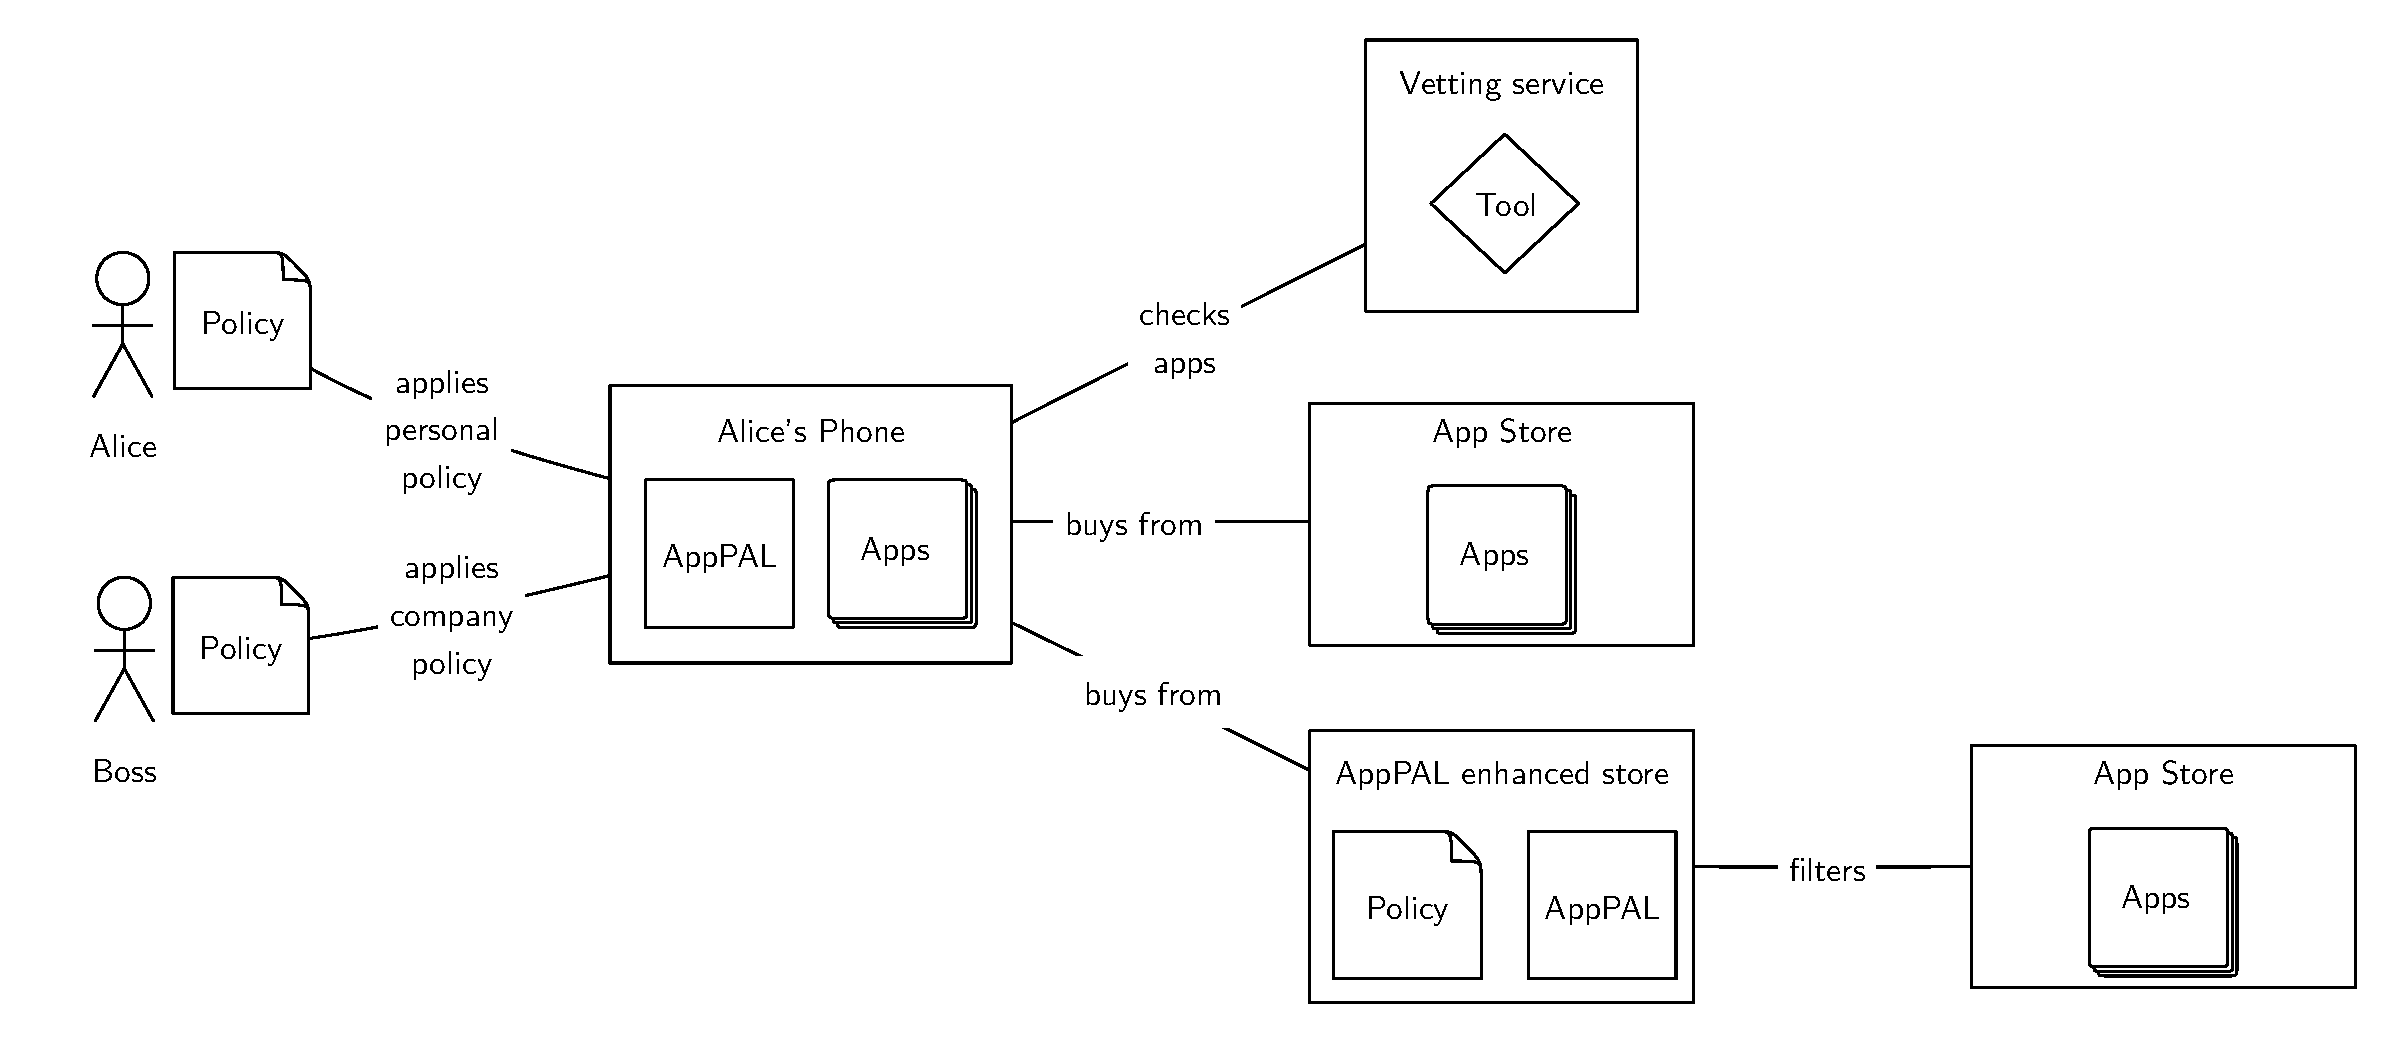
\includegraphics{figures/overview.eps}
\caption{Ecosystem of devices and stores with AppPAL.}
\label{fig:ecosystem}
\end{figure}

We propose a change to the ecosystem, shown in \autoref{fig:ecosystem}.
People have policies which are enforced by AppPAL on their devices.
They can be composed with policies from employers or others to create enhanced devices that ensure apps meet the policies of their owners.
The device can make use of vetting services which run tools to infer complex properties about apps.
Users can buy from enhanced stores which ensure the only apps they sell are the apps which meet the explicitly specified store policies.
Developers could decide which stores to sell their apps in on the basis of policies about stores.

\section{Expressing policies in AppPAL}
\label{sec:idea}

In \autoref{sec:problem} Alice and Emma had policies they wanted to enforce but no means to do so.
Instead of using several different tools to enforce Emma's policy disjointedly, we could use an authorization logic.
In \autoref{lst:corporate} we give an AppPAL policy implementing Emma's app concerns on Alice's phone.
% A pictorial representation, is given in \autoref{fig:emmas_policy}; color splits statements by each speaker.

SecPAL is a logic of authorization for access control decisions in distributed systems.
It has a clear and readable syntax, as well as rich mechanisms for delegation and constraints.
SecPAL has already been used as a basis for other policy languages in areas such as privacy preferences~\cite{Becker:2009ula} and data-sharing~\cite{Aziz:2011vt}.
We present AppPAL as a modified form of SecPAL, targeting apps on mobile devices.

\begin{figure}
  \begin{minipage}[t]{0.5\textwidth}
    \begin{lstlisting}[numbers=left,
                       escapeinside={@}{@},
                       basicstyle=\scriptsize\ttfamily,
                       stringstyle=\scriptsize\sffamily,
                       keywordstyle=\scriptsize\slshape]
"alice" says "emma" can-say inf
  App isRunnable. @\label{lst:corporate_1}@

"emma" says App isRunnable @\label{lst:corporate_2}@
  if "no-tracking-policy" isMetBy(App),
     "reputable-policy" isMetBy(App),
     "anti-virus-policy" isMetBy(App).

"emma" says
  "reputable-policy" isMetBy(App) @\label{lst:corporate_3}@
      if App isReputable.

"emma" says "google-play" can-say 0
  App isReputable. @\label{lst:corporate_4}@
    \end{lstlisting}
  \end{minipage}\begin{minipage}[t]{0.5\textwidth}
    \begin{lstlisting}[numbers=left,
                       escapeinside={@}{@},
                       firstnumber=15,
                       basicstyle=\scriptsize\ttfamily,
                       stringstyle=\scriptsize\sffamily,
                       keywordstyle=\scriptsize\slshape]
"emma" says "anti-virus-policy" isMetBy(App) @\label{lst:corporate_5}@
  if App isAnApp
  where
    mcAfeeVirusCheck(App) = false.

"emma" says "no-location-permissions"
  can-act-as "no-tracking-policy". @\label{lst:corporate_6}@

"emma" says
  "no-location-permissions" isMetBy(App) @\label{lst:corporate_7}@
    if App isAnApp
    where
      hasPermission(App, "LOCATION")=false.
\end{lstlisting}
\end{minipage}
\caption{AppPAL policy implementing Emma's security requirements}
\label{lst:corporate}
\end{figure}

In \autoref{lst:corporate_1} Alice gives Emma the ability to specify whether an \code{App} (a variable) \code{isRunnable} (a predicate).
She allows her to delegate the decision further if she chooses (\code{can-say inf}).
Next in \autoref{lst:corporate_2} Emma specifies her concerns as policies to be met (the \code{isMetBy()} predicate that takes an app as its argument).
If Emma can be convinced all these policies are met then she will say the \code{App isRunnable}.
In \autoref{lst:corporate_3} and \autoref{lst:corporate_4} Emma specifies that an app meets the \code{reputable-policy} if the \code{App isReputable};
  with \code{"google-play"} specified as the decider of what is buyable or not.
This time Google is not allowed to delegate the decision further (\code{can-say 0}).
In other words Google is not allowed to specify Amazon as a supplier of apps as well.
Google must say what is buyable directly for Emma to accept it.
Emma specifies the \code{"anti-virus-policy"} in \autoref{lst:corporate_5}.
Here we use a constraint.
When checking the policy the \code{mcAfeeVirusCheck} should be run on the \code{App}.
Only if this returns \code{false} will the policy be met.
To specify the \code{"no-tracking-policy"} Emma says that the \code{"no-location-permissions"} rules implement the \code{"no-tracking-policy"} (\autoref{lst:corporate_6}).
Emma specifies this in \autoref{lst:corporate_7} by checking the app is missing two permissions.

Alice wants to install a new app (\code{com.facebook.katana}) on her phone.
To meet Emma's policy the AppPAL checker needs to collect statements to show the app meets the \code{isRunnable} predicate.
Specifically it needs:
\begin{itemize}
  \item\code{"emma" says "com.facebook.katana" isAnApp.}
    A simple typing statement that can be generated for all apps as they are encountered.
    This helps keep the number of assertions in the policy low aiding readability.
  \item\code{"google-play" says "com.facebook.katana" isReputable.}
    Required to convince Emma the app came from a reputable source.
    It should be able to obtain this statement from the Play store as the app is available there.
  \item\code{"emma" says "anti-virus-policy" isMetBy("com.facebook.katana").}
    She can obtain this by running the \ac{av} program on her app.
  \item\code{"emma" says "no-locations-permissions" isMetBy("com.facebook.katana").}
    Needed to show the App meets Emma's no-tracking-policy.
    Emma will say this if after examining the app the location permissions are missing.
\end{itemize}
These last two statements require the checker to do some extra checks to satisfy the constraints.
To get the third statement it must run the \ac{av} program on her app and check the result.
The results from the \ac{av} program may change with time as it's signatures are updated;
  so the checker must re-run this check every time it wants to obtain the statement connected to the constraint.
For the forth statement the checker needs to check the permissions of the app.
It could do this by looking in the \texttt{MANIFEST.xml} inside the app itself, or through the Android package manager if it is running on a device.

In this scenario we have imagined Alice wanting to check the apps as she installs them.
We could also imagine Emma wanting a personalised app store where all apps sold meet her policy.
With AppPAL this can be implemented by taking an existing store and selectively offering only the apps which will meet the user's policy.
This gives us a \emph{filtered store} which, from an existing set of apps, we get a personalised store that only sells apps that meet a policy.

\section{AppPAL}
\label{sec:details}
\label{ssec:language}

AppPAL is implemented as a library for Android and Java.
The parser is implemented using ANTLR4.
The structure of an AppPAL assertion can be seen in \autoref{fig:assertion}.

\begin{figure}
  \newcommand{\bracetext}[1]{\text{\sffamily #1}}
  \newcommand{\smalltext}[1]{\text{\ttfamily\footnotesize #1}}
  \centering
  \begin{equation*}\small
    \begin{array}{r l}\footnotesize
      \overbrace{\smalltext{"user"}}^{\bracetext{speaker}} &
      \smalltext{ says }\overbrace{\overbrace{\smalltext{ App }}^{\bracetext{subject}}\overbrace{\smalltext{ isRunnable}}^{\bracetext{predicate}}}^{\bracetext{fact}} \\
      & \overbrace{\smalltext{ if App isFree}}^{\bracetext{condition}} \\
      & \overbrace{\smalltext{ where hasPermission(App, "INTERNET") = true}}^{\bracetext{constraint}}.
    \end{array}
  \end{equation*}
  \caption{Structure of an AppPAL assertion.}
\label{fig:assertion}
\end{figure}

In Becker~\etal's work~\cite{Becker:2006vh} they leave the choice of predicates, and constraints for their SecPAL open.
With AppPAL we make explicit our predicates and how they relate to Android.
AppPAL policies can make use of the predicates and constraints in \autoref{tab:predicates}.
Additional predicates can be created in the policy files, but adding or modifying constraints required a code change\footnote{The Android version of the \texttt{hasPermission} constraint, for example, uses the Android package manager to determine what permissions an app requests, but the Java version uses the Android platform tools.  This requires a small code change.}

\begin{table}
\begin{tabulary}{\linewidth}{l L}
  \toprule
  Name & Description \\
  \midrule
  App \texttt{isRunnable} & Says an app can be run. \\
  App \texttt{isInstallable} & Says an app can be installed. \\
  App \texttt{isAnApp} & Tells AppPAL that an app exists. \\
  Policy \texttt{isMetBy(}App\texttt{)} & Says a specific policy is met by an app.  This is used to split policies into smaller components which can be reused and composed. \\
  \texttt{hasPermission(}App, Permission\texttt{)} & Constraint for testing whether an app has been granted a permission. \\
  \texttt{BeforeHourOfDay(}time\texttt{)} & Constraint used to test whether we're before an hour in the day. \\
  Tool\texttt{Check(}App, Property) &  General form of a constraint used to run a static analysis tool over an app. \\
  \bottomrule
\end{tabulary}
\caption{Typical AppPAL predicates and constraints}
\label{tab:predicates}
\end{table}



% \begin{description}
%   \item[\texttt{App isRunnable}]
%     Used to indicate that an App meets the install policy for the device.
%     Showing an app satisfies this predicate is usually the goal of evaluating AppPAL.
%
%   \item[\texttt{App isAnApp}]
%     Expresses a simple typing relations.
%     AppPAL, and SecPAL, have a safety condition that all variable mentioned in the fact, are also mentioned in the condition body (as is the case for Datalog and other logic languages).
%     These typing relations allow an appeal to ground facts to be made so the safety condition is satisfied.
%     This typically is necessary when an assertion has a constraint but no body conditions: we add the trivial typing statement to the body to ensure the assertion is accepted by AppPAL.
%
%   \item[\texttt{Policy isMetBy(App)}]
%     Policies let you split app behaviour into sub-policies.
%     For example in \autoref{sec:idea} we showed how Emma's installation policy could be written using three \texttt{isMetBy} statements.
%     Splitting policies allows greater control of how each one is checked.
%     We can delegate checking a policy to an expert using the \code{can-say} statement.
%     We can specify more detailed checks using the \code{can-act-as} statements.
%
%   \item[\texttt{Policy shownIsMetBy(Evidence, App)}]
%     A variant of the \texttt{isMetBy} statement that allows some evidence (a proof) to be given that shows the policy is met.
% \end{description}

Splitting the decision about whether an app is runnable into a series of policies that must be met gives us flexibility in how the decision is made.
It allows us to describe multiple means of making the same decision, and provide backup routes when one fails.
Some static analysis tools are not quick to run.
Even taking minutes to run a battery draining analysis can be undesirable.
If a user wants to download an app quickly they may not be willing to wait to check that a policy is met.

In \autoref{sec:problem} and \autoref{sec:idea} we described a \emph{no-tracking-policy} to prevent a user's location being leaked.
In Emma's policy we checked this using the app's permissions.
If the app couldn't get access to the GPS sensors (using the permissions) then it met this policy.
Some apps may want to access this data, but may not leak it.
We could use a taint analysis tool to detect this (e.g.~Taintdroid~\cite{Fritz:2013vi}).
Our policy now becomes:

\begin{lstlisting}
"emma" says "no-locations-permissions"
  can-act-as "no-tracking-policy".

"emma" says "no-locations-permissions" isMetBy(App)
  if App isAnApp
  where
    hasPermission(App, "ACCESS_FINE_LOCATION") = false,
    hasPermission(App, "ACCESS_COARSE_LOCATION") = false.

"emma" says "location-taint-analysis"
  can-act-as "no-tracking-policy".

"emma" says "location-taint-analysis" isMetBy(App)
  if App isAnApp
  where
    taintDroidCheck(App, "Location", "Internet") = false.
\end{lstlisting}

Sometimes we might want to use location data.
For instance Emma might want to check that Alice is at her office.
Emma might track Alice using a location tracking app.
Provided the app only talks to Emma, and it uses SSL correctly (which Mallodroid can check for~\cite{Fahl:2012dj}) she is happy to relax the policy.

\begin{lstlisting}
"emma" says "relaxed-no-tracking-policy" canActAs "no-tracking-policy".
"emma" says "relaxed-no-tracking-policy" isMetBy(App)
  if App hasCategory("tracking")
  where
    mallodroidSSLCheck(App) = false,
    connectionsCheck(App, "[https://emma.com]") = true.
\end{lstlisting}

This gives us four different ways of satisfying the \emph{no-tracking-policy}:
  with permissions,
  with taint analysis,
  with a relaxed version of the policy,
  or by Emma directly saying the app meets it.
When we come to check the policy if any of these ways give us a positive result we can stop our search.

% AppPAL also helps attribute blame when things go wrong.
% By modelling the trust relationships in systems we can work out precisely where mistakes were made.
% A recent example demonstrating this is \textsc{CVE-2015-2077}.
% Lenovo was found to be shipping laptops with the \emph{Superfish} malware pre-installed.
% Lenovo had also installed an \ac{av} package on their laptops; this \ac{av} did recognise Superfish as malware.
% Unfortunately they had configured it to ignore Superfish.
% The malware was an ad framework designed to show users products similar to those they viewed on the web.
% Unfortunately it did so by man-in-the-middling all SSL traffic using a shared private key.
%
% From a user's perspective there was a delegation of trust to Lenovo to detect malware.
% Lenovo then delegated further to McAfee to supply the antivirus checking; but left an exception that they would allow Superfish.
% A user might wonder where the breach of trust occurred and who is to blame?
% Is it the \ac{av} failing to spot the malware?
% Has someone else configured the software incorrectly?
% How should they fix the problem?
%
% If we write this in the AppPAL policy language the cause of the breach of trust becomes apparent; as does the fix.
% \begin{lstlisting}[numbers=left, escapeinside={@}{@}, label={lst:lenovo}]
% "user" says "lenovo" can-say inf File isSafe. @\label{lst:lenovo_trust}@
% "lenovo" says "mcafee" can-say inf File isSafe.
% "lenovo" says "C:\System\superfish" isSafe. @\label{lst:lenovo_unsafe}@
% \end{lstlisting}
% The fault lies with \autoref{lst:lenovo_unsafe}.
% Lenovo has caused the problem (they \emph{said} it was safe).
% The fix is to revoke this statement, or to revoke \autoref{lst:lenovo_trust} and find a different \ac{av} supplier.

\subsection{Policy checking}
\label{ssec:eval}

AppPAL has the same policy inference rules as SecPAL.
We do not use Becker~\etal's DatalogC~\cite{Li:2003ix}~based checking algorithm, as no DatalogC library exists for Android.
We have implemented the rules directly in Java.
Pseudo-code is given in \autoref{fig:pseudocode}.

Like Becker~\etal~we make use of an assertion context to store known statements.
We also cache intermediate results, and ground facts to avoid re-computation.
On a mobile device memory is at a premium.
We would like to keep the context as small as possible.
For some assertions (like \code{isAnApp}) we derive them by checking the arguments at evaluation time.
This gives us greater control of the evaluation and how the assertion context is created.
For example, when checking the \code{isAnApp} predicate;
  we can fetch the assertion that the subject is an app based on the app in question.
Similarly when we use a statement from \emph{Emma} that \emph{Google-Play can-say} whether an app is buyable;
  it is sensible to go fetch from the store whether the app is saleable and make Google say it then and there.

% In SecPAL there is no type.
% All entities are either constants (implemented as strings) or variables.
% There is no differentiation made between a \emph{voiced} constant (who says assertions),
% and a \emph{subject} (the subject of a verb-phrase, or predicate argument).
% In AppPAL the subjects are usually apps or policies.
% Apps do not utter facts;
%   so there is no need to check them as potential speakers of \emph{can-say} statements.
% Similarly if a constant never appears as a subject of a statement, as most speakers do not,
%   there is no need to check it as a possible subject for a \emph{can-act-as} statement.
% We pre-process the assertion context to find \emph{voiced} and \emph{subject} constants.
% This means we need to search less constants when attempting to replace a variable, speeding evaluation.

\begin{figure}\centering
\begin{minipage}[b]{0.49\linewidth}
\begin{lstlisting}[language=Ruby, basicstyle=\ttfamily\scriptsize, keywordstyle=\scriptsize\slshape, columns=flexible]
def evaluate(ac, rt, q, d)
  return rt[q, d] if rt.contains q, d
  p = cond(ac, rt, q, d)
  if p.isValid then
    return (Proven, rt.update q, d, p)
  p = canSay_CanActAs(ac, rt, q, d)
  if p.isValid then
    return (Proven, rt.update q, d, p)
  else
    return (Failure, rt.update q, d, Failure)
\end{lstlisting}
\end{minipage}
\begin{minipage}[b]{0.49\linewidth}
\begin{lstlisting}[language=Ruby, basicstyle=\ttfamily\scriptsize, keywordstyle=\scriptsize\slshape, columns=flexible]
def canSay_CanActAs(ac, rt, q, d)
  ac.constants.each do |c|
    if c.is_a :subject
      p = canActAs ac, rt, q, d
      return Proven if p.isValid
    elsif c.is_a :speaker
      p = canSay ac, rt, q d
      return Proven if p.isValid
  return Failure
\end{lstlisting}
\end{minipage}

\begin{minipage}[b]{0.49\linewidth}
\begin{lstlisting}[language=Ruby, basicstyle=\ttfamily\scriptsize, keywordstyle=\scriptsize\slshape, columns=flexible]
def cond(ac, rt, q, d)
  ac.add q.fetch if q.isFetchable
  ac.assertions.each do |a|
    if (u = q.unify a.consequent) &&
       (a = u.substitution a).variables == none
      return checkConditions ac, rt, a, d
  return Failure
\end{lstlisting}
\end{minipage}
\begin{minipage}[b]{0.49\linewidth}
\begin{lstlisting}[language=Ruby, basicstyle=\ttfamily\scriptsize, keywordstyle=\scriptsize\slshape, columns=flexible]
def checkConditions(ac, rt, a, d)
  getVarSubs(a,ac.constants).each do |s|
    sa = s.sub a
    if sa.antecedents.all
        { |a| evaluate(ac, rt, a, d).isValid }
      p = evaluateC sa.constraint
      return Proven if p.isValid
  return Failure
\end{lstlisting}
\end{minipage}
\caption{Partial-pseudocode for AppPAL evaluation.}
\label{fig:pseudocode}
\end{figure}

% \subsection{Policy Examples}
% \label{ssec:idioms}
%
% When writing policies some schemes often come up.
% We give examples of policies and queries and show how they can be implemented in AppPAL.
%
% \begin{description}
%   \item[Policies for home and work]
%     In \autoref{sec:introduction} we said Alice might like to have separate rules for home and work.
%     Emma may insist that her policies come into effect whenever Alice is at work, but is okay with Alice breaking them after 5~pm or when she isn't at work.
%     To implement this we add rules that use constraints to decide whether an app should be run.
%     Alice already has the Emma's work policy as the default.
%     Now she just needs to add an exception to the rule.
%     \begin{lstlisting}
% "alice" says App isRunnable
%   if "home-policy" isMetBy(App)
%   where TimeOfDay() > 17.00.
%
% "alice" says App isRunnable
%   if "home-policy" isMetBy(App)
%   where At("work") = false.
%     \end{lstlisting}
%
%   \item[App white-listing by an IT department]
%     Inside Emma's company employees in the IT department may white-list certain apps as runnable.
%     Emma delegates to them to decide if an app is runnable.
%     \begin{lstlisting}
% "emma" says "it-department" can-say 0 App isRunnable.
%     \end{lstlisting}
%     Charlie and Diveena work in the IT department.
%     When they have checked an app they say it is runnable.
%     \begin{lstlisting}
% "emma" says "charlie" can-act-as "it-department".
% "emma" says "diveena" can-act-as "it-department".
%
% "charlie" says "com.facebook.katana" isRunnable.
% "diveena" says "org.thoughtcrime.securesms" isRunnable.
%     \end{lstlisting}
%
%   \item[Overpriviliged applications]
%     Alice is particularly worried about apps stealing her data.
%     She knows that certain apps need certain permissions.
%     For example a photography app needs access to the camera.
%     She checks each app's permissions carefully for things that seem unusual.
%
%     Alice's policy can be implemented by checking the permissions of the app, using constraints.
%     \begin{lstlisting}
% "alice" says App isRunnable
%    if "permissions-policy" isMetBy(App).
% "alice" says "permissions-policy" isMetBy(App)
%    if App isAnApp
%    where
%       category(App, "Photography"),
%       hasPermission(App, "LOCATION") = false,
%       hasPermission(App, "CAMERA") = true.
%     \end{lstlisting}
%
%     Discovering the \emph{normal} permissions for an app can be done by mining large stores of apps, or apps a user has previously installed.
%     Alternately tools like Stowaway~\cite{Felt:2011kj} could be integrated to check apps.

%   \item[Digital Evidence]
%     In \autoref{ssec:language} we described how digital evidence could be used to decide if policies are met.
%     Suppose a digital evidence generating tool, such as \emph{Evicheck}, can be used to check a policy.
%     For example that no audio can be recorded without the users consent~\cite{Seghir:2014uq}.
%     Using this tool someone generates a proof certificate that this property is met.
%     This might be the developer of the app, a third party certification service, or someone else;
%       when we check the proof we will discover if it is valid or not.
%     \begin{lstlisting}
% "alice" says Anyone can-say 0
%   "recording-consent" shownIsMetBy(Evidence, App).
%
% "skb" says "recording-consent"
%   shownIsMetBy("evicheck://evidence123", App).
%
% "alice" says "recording-consent" isMetBy(App)
%   if "recording-consent" shownIsMetBy(Evidence, App)
%   where
%     evicheckCheckEvidence(Evidence, App) = true.
%     \end{lstlisting}
%     In the example here Alice allows anyone to present her with evidence for her policy.
%     A \ac{skb} offers some evidence, and Alice accepts it as if it checks out.
% \end{description}

\subsection{Benchmarks}
\label{ssec:benchmarks}

We envisage AppPAL running on a mobile phone checking apps.
For it to be a viable solution the policy checking performance must be reasonable: capable of checking apps against a policy as quickly as possible.
The policy checking search procedure is at its slowest when performing large repeated delegations.
Two synthetic benchmarks were created to check that the search procedure performed acceptably.
Each benchmark consisted of a repeated chain of delegations.
The \emph{straight} benchmark consists of a single long chain of delegation.
The \emph{forking} benchmark consists of a binary tree of principals delegating to each other.
These benchmarks are reasonable as they model the worst kinds of policies to evaluate---though worse ones could be designed by forking even more.
A snippet of each policy is shown in \autoref{fig:policy-snippet}.

On a \emph{Nexus 4} checking times are measured in seconds when there are hundreds of delegations, and in minutes when there are thousands (\autoref{fig:benchmarks}).
We have only used a few delegations per decision when describing hypothetical user policies.
Since the benchmarks show that long chains of delegation can be used, we believe the performance is acceptable.

\begin{figure}\centering
  \begin{minipage}{0.49\linewidth}
    \begin{lstlisting}[basicstyle=\ttfamily\scriptsize, keywordstyle=\ttfamily\slshape\scriptsize]
    '1' says '2' can-say App isInstallable.
    '2' says '3' can-say App isInstallable.
    '3' says '4' can-say App isInstallable.
    '4' says '5' can-say App isInstallable.
    '5' says '6' can-say App isInstallable.
    '6' says '7' can-say App isInstallable.
    \end{lstlisting}
  \end{minipage}
  \begin{minipage}{0.49\linewidth}
    \begin{lstlisting}[basicstyle=\ttfamily\scriptsize, keywordstyle=\ttfamily\slshape\scriptsize]
    '1' says '2' can-say App isInstallable.
    '1' says '3' can-say App isInstallable.
    '2' says '4' can-say App isInstallable.
    '2' says '5' can-say App isInstallable.
    '3' says '6' can-say App isInstallable.
    '3' says '7' can-say App isInstallable.
    \end{lstlisting}
  \end{minipage}
  \caption{Straight and forking policies used for benchmarking.}
  \label{fig:policy-snippet}
\end{figure}

\begin{figure}
  \begin{minipage}{0.49\linewidth}
    \begin{tabular}{c c c c}
       \toprule
       Policy   & Nodes & Parse (s) & Check (s) \\
       \midrule
       Straight & 10    & 0.01      & 0.04      \\
       Straight & 100   & 0.05      & 1.00      \\
       Straight & 500   & 0.32      & 21.07     \\
       Straight & 1000  & 0.43      & 87.75     \\
       \midrule
       Forking  & 256   & 0.10      & 1.93      \\
       Forking  & 512   & 0.23      & 7.47      \\
       Forking  & 1024  & 0.45      & 28.29     \\
       Forking  & 2048  & 0.85      & 117.68    \\
       \bottomrule
    \end{tabular}
  \end{minipage}
  \begin{minipage}{0.49\linewidth}
    \includegraphics[width=\linewidth]{figures/benchmarks.eps}
  \end{minipage}
  \caption{Benchmarking results on a Nexus 4 Android phone.}
  \label{fig:benchmarks}
\end{figure}

\section{Demonstration}
\label{sec:demonstation}

Throughout we have asserted that user's have policies and that there is a need for policy enforcement tools.
Corporate mobile security \ac{BYOD policies} have started appearing and NIST have issued recommendations for writing them~\cite{Scarfone:2009vy,Souppaya:2013jf}.
In a study of 725 Android users, Lin~\etal~found four patterns that characterise user privacy preferences for apps~\cite{Sadeh:2014vq}.
Using app installation data from Carat~\cite{Oliner:2013ht} we used AppPAL to find the apps satisfying each policy Lin~\etal~identified and measured the extent each user was following them.

Lin~\etal~identified four types of user.
The \emph{Conservative} (C) users were uncomfortable allowing an app access to any personal data for any reason.
The \emph{Unconcerned} (U) users felt okay allowing access to most data for almost any reason.
The \emph{Advanced} (A) users were comfortable allowing apps access to location data but not if it was for advertising reasons.
Opinions in the largest cluster, \emph{Fencesitters} (F), varied but were broadly against collection of personal data for advertising purposes.
We wrote AppPAL policies to describe each of these behaviours as increasing sets of permissions.
These simplify the privacy policies identified as by Lin~\etal~as we do not take into account the reason each app might have been collecting each permission.

\newcommand{\tabtitle}[1]{\textbf{\footnotesize #1}}
\begin{center}
  \begin{tabular}{ r l l l l }
%                                       & \rothead{Conservative} & \rothead{Advanced} & \rothead{Fencesitter} & \rothead{Unconcerned} \\
    \toprule
    \tabtitle{Policy}                  & \tabtitle{C}           & \tabtitle{A}       & \tabtitle{F}          & \tabtitle{U}          \\
    \midrule
    \lstinline{GET_ACCOUNTS}           & \xmark                 & \xmark             & \xmark                & \xmark                \\
    \lstinline{ACCESS_FINE_LOCATION}   & \xmark                 & \xmark             & \xmark                &                       \\
    \lstinline{READ_CONTACT}           & \xmark                 & \xmark             & \xmark                &                       \\
    \lstinline{READ_PHONE_STATE}       & \xmark                 & \xmark             &                       &                       \\
    \lstinline{SEND_SMS}               & \xmark                 & \xmark             &                       &                       \\
    \lstinline{ACCESS_COARSE_LOCATION} & \xmark                 &                    &                       &                       \\
    \bottomrule
  \end{tabular}
\end{center}

Malware is available for Android.
Like other vendors, McAfee classify malware into several categories.
The \emph{malicious} and \emph{trojan} categories describe traditional malware.
Other categories classify \ac{pup} such as aggressive adware.
Using AppPAL we can write policies to differentiate between different kinds of malware, characterising users who allow dangerous apps and those who install poor quality ones.
\begin{lstlisting}
"user" says "mcafee" can-say
  "malware" isKindOf(App).
"mcafee" says "trojan" can-act-as "malware".
"mcafee" says "pup" can-act-as "malware".
\end{lstlisting}
If a user is enforcing a privacy policy we might also expect them to install less malware.
We can check this by using AppPAL policies to find the malware and again measure the number of malwares each user had installed.

We want to test how well policies capture user behaviour.
Installation data was taken from a partially anonymized\footnote{Users are replaced with incrementing numbers, app names are replaced with hashes to protect sensitive names.} database of installed apps captured by Carat~\cite{Oliner:2013ht}.
By calculating the hashes of known package names we see who installed what.
The initial database has over 90,000 apps and 55,000 users.
On average each user installed around 90 apps each; 4,300 apps have known names.
Disregarding system apps (such as \texttt{com.android.vending}) and very common apps (Facebook, Dropbox, Whatsapp, and Twitter) we reduced the set to an average of 20 known apps per user.
To see some variations in app type, we considered only the 44,000 users who had more than 20 known apps.
Using this data, and the apps themselves taken from the Google Play Store and Android Observatory~\cite{Barrera:2012iba}, we checked which apps satisfied which policies.

\begin{figure}\centering
  \subfigure[Use of policies modelling user behaviour.]{%
    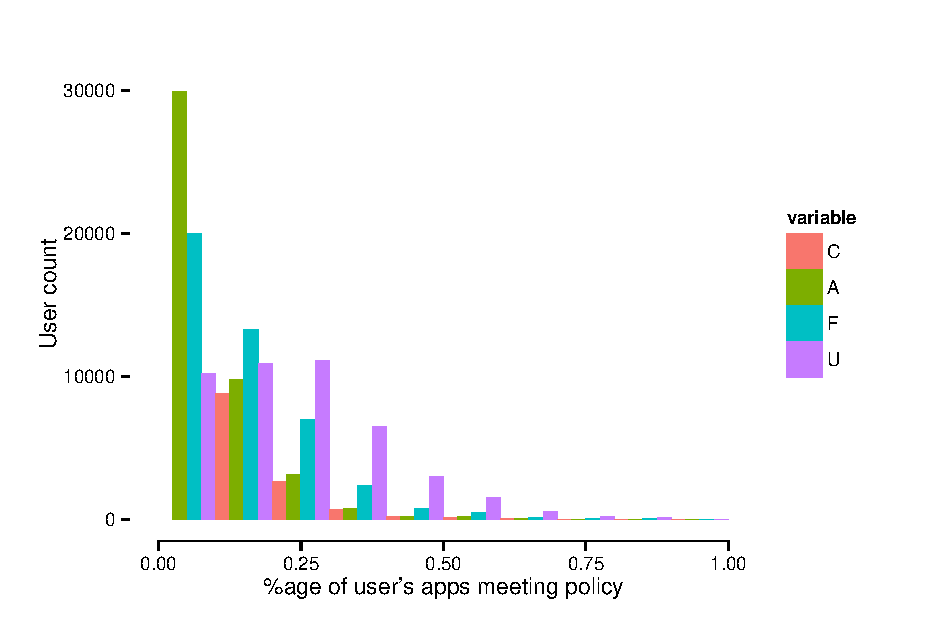
\includegraphics[width=0.48\linewidth]{./figures/lin.eps}
    \label{fig:lin}}
  \subfigure[Percentage of malware in installed apps for users installing some malicious apps.]{%
    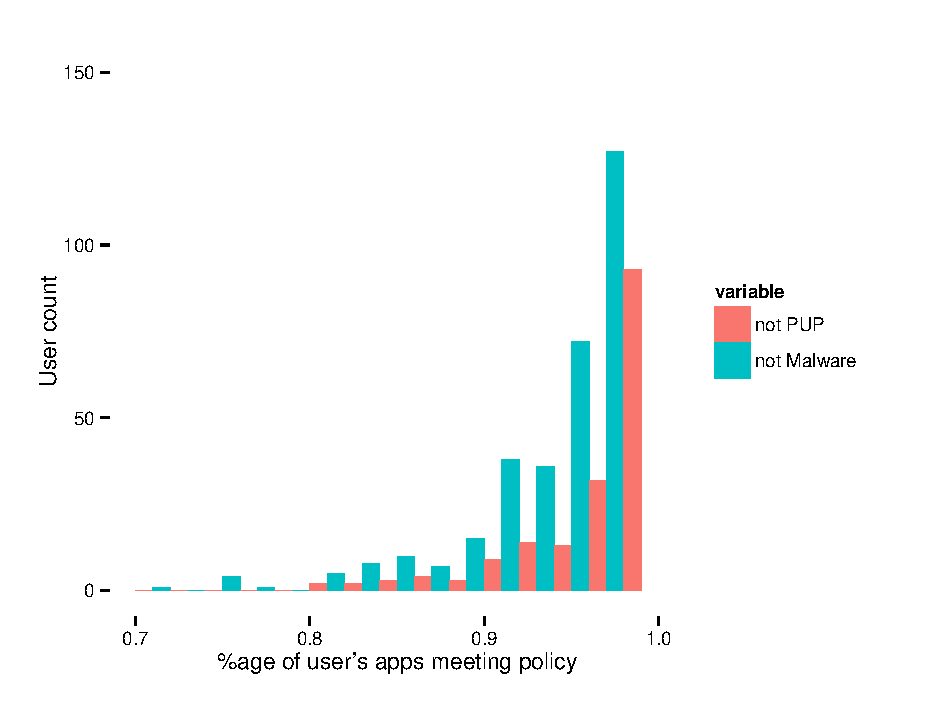
\includegraphics[width=0.48\linewidth]{./figures/malware.eps}
    \label{fig:malware}}
  \caption{Policy compliance graphs.}
\end{figure}

Figure~\ref{fig:lin} shows that very few users follow Lin~\etal's policies most of the time.
Whilst the AppPAL policy we used was a simplified version of Lin~\etal's policy, it suggests that there is a disconnect between users privacy preferences and their behaviour (often referred to as the \emph{privacy paradox}).
A few users, however, did seem to be installing apps meeting these policies most of the time.
This suggests that while users may have privacy preferences the majority are not attempting to enforce them.
Policy enforcement tools, like AppPAL, can help users enforce their own policies which they cannot do easily using the current means available to them.

\begin{figure}\centering
  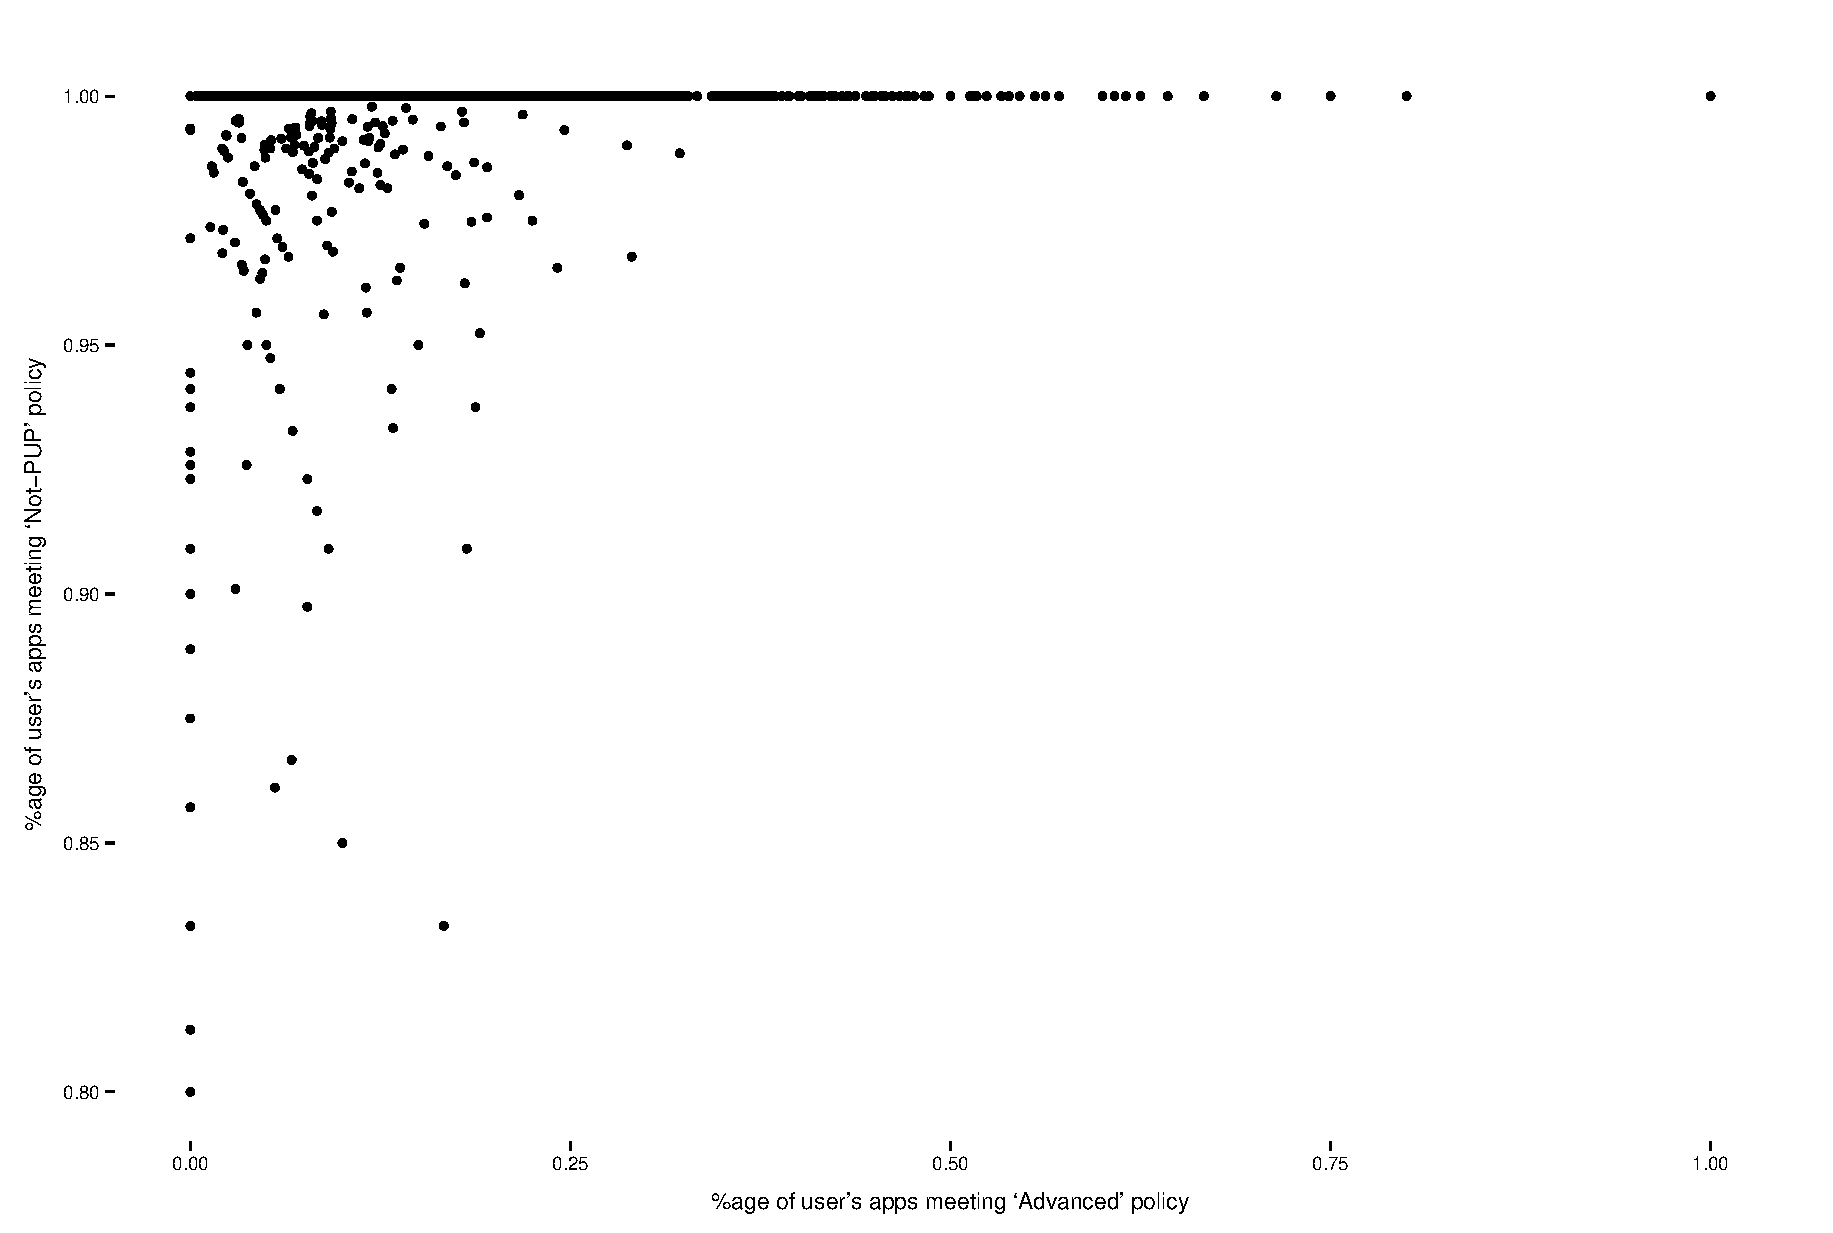
\includegraphics[width=0.5\linewidth]{./figures/c_v_pup.eps}
  \caption{Compliance with the advanced policy and non-\ac{pup} policy.}
  \label{fig:versus}
\end{figure}

We found 1\% of the users had a \ac{pup} or malicious app installed.
Figure~\ref{fig:malware} shows that infection rates for \ac{pup}s and malware is low;
though a user is 3 times more likely to have a \ac{pup} installed than malware.
Users who were complying more than half the time with the conservative or advanced policies complied with the malware or \ac{pup} policies fully (\autoref{fig:versus}).
This suggests that policy enforcement is worthwhile: users who can enforce policies about their apps experience less malware.
%This is significant (P-value $< 0.05$) and suggests that users who pick their apps carefully are less likely to experience malware.

Using AppPAL we have written short policies describing user behaviour and used these to identify the users following them to varying degrees.
Some limitations of our results include:
\begin{itemize}
\item
  We do not have the full user purchase history, and we can only find out about apps whose names match those in available databases.
  So a user may have apps installed that break the policy without us knowing.
\item
  Recently downloaded apps used for experiment may not be the same version that users had, in particular, their permissions may differ.
  Permissions tend to increase in apps over time~\cite{Wei:2012id}; so a user may be more conservative than our analysis suggests.
\item
  The AppPAL policies we used are a simplification of the identified privacy preferences.
  User's could be following policies more nuanced than our implementation.
  We believe our approximation is valid, however, as users will not know the precise reason an app uses a permission, and may decline to install it anyway.
  Our policies could be made more precise by incorporating the app category, and allowing apps to have a permission when it is appropriate (i.e.~a text messaging client will need the \texttt{SEND_SMS} permission to run).
\end{itemize}

\section{Related work}

Authorization logics have been successfuly used to enforce policies in several other domains.
The earliest such logic, PolicyMaker~\cite{Blaze:dj}, was general, if undecidable.
Logics that followed like KeyNote~\cite{Blaze:1999fa} and SPKI/SDSI~\cite{Ellison:1999ui} looked at public key infrastructure.
The RT-languages~\cite{Li:2002if,Li:2003ix,Li:2003to} were designed for credential management.
Cassandra~\cite{Becker:2004fi} was used to model trust relationships in the british national health service.

SELinux is used to describe policies for Linux processes, and for access control (on top of the Linux discretionary controls).
It was ported to Android~\cite{Smalley:2013vl} and is used in the implementation of the permissions system.
Google also offer the \emph{Device Policy for Android} app.
This lets businesses configure company owned devices to be trackable, remote lockable, set passwords and sync with their servers.
It cannot be used to describe policies about apps, or describe trust relationships, however.

The SecPAL language is designed for access control in distributed systems.
We picked SecPAL as the basis for AppPAL because it was readable, extensible, and seemed to be a good fit for the problem we were trying to solve~\cite{Hallett:2014un}.
It has already been used to describe data usage policies~\cite{Aziz:2011vt} and inside Grid data systems~\cite{Humphrey:2007wc}.
Other work on SecPAL has added various features such as existential quantification~\cite{Becker:2009vt} and ultimately spawned the DKAL family of policy languages~\cite{Gurevich:2008fz,Gurevich:Qo5E3M3}.
Gruevich and Neeman showed that SecPAL was a subset of DKAL (minus the \emph{can-act-as} statement).
DKAL also contains more modalities than \emph{says}, which lets policies describe actions principals carry out rather than just their oppinions.
For example in AppPAL a user might \emph{say} an app is installable if they would install it (\code{"user" says App isInstallable})
In DKAL they can describe the conditions that would force them to install it (\code{"user" installs App}).
The distinction is that in AppPAL whilst the user thinks the app could be installed we do not know for sure whether the user has installed it.
With DKAL we can guarantee that the action was completed.

Kirin~\cite{Enck:2009ko} is a policy language and tool for enforcing app installation policies preventing malware.
Policy authors could specify combinations of permissions that should not appear together.
For example an author might wish to stop malware sending premium rate text messages.
To might implement this by restricting an app having both the \texttt{SEND\_SMS} and \texttt{WRITE\_SMS} permissions (\autoref{fig:kirin}).
Using this approach they found vulnerabilities in Android, but were ultimately limited by being restricted to permissions and broadcast events.
\begin{figure}
\begin{lstlisting}
restrict permission [SEND_SMS] and permission [WRITE_SMS]
\end{lstlisting}
% \begin{lstlisting}
% "user" says "no-write-send-sms" isMetBy(App)
%   where hasPermission(App, "SEND_SMS") = false.
% "user" says "no-write-send-sms" isMetBy(App)
%   where hasPermission(App, "WRITE_SMS") = false.
% \end{lstlisting}
\caption{Kirin policy stopping apps monetized by premium rate text messages.}
\label{fig:kirin}
\end{figure}

This approach could help identify malware, but it is less suitable for detecting \acp{pup}.
The behaviours and permissions \ac{pup} displays aren't necessarily malicious.
One user may consider apps which need in-app-purchases to play malware, but another may enjoy them.
With Kirin we are restricted to permitting or allowing apps.
AppPAL is more general: we can describe more scenarios than just permit or allow, and use more app information than just permissions.
By allowing delegation relationships we can understand the provenance and trust relationships in these rules.
With AppPAL we can incorporate static analysis results and take into account the user's location and other constraints.

There has been a great amount of work on developing app analysis tools for Android.
Tools such as Stowaway~\cite{Felt:2011kj} detect overprivileged apps.
TaintDroid~\cite{Enck:2010uw} and FlowDroid~\cite{Fritz:2013vi} can do taint and control flow analysis; sometimes even between app components.
Other tools like QUIRE~\cite{Bugiel:2012ui} can find privilege escalation attacks between entire apps.
ScanDAL~\cite{Kim:2012vt} and SCanDroid~\cite{Fuchs:2009vi} help detect privacy leaks.
Appscopy~\cite{Feng:kPGZr_ja} searches for specific kinds of malware.
Tools like DroidRanger~\cite{Zhou:2012tb} scan app markets for malicious apps.
Many others exist checking and certifying other aspects of app behaviour.

\section{Conclusions and further work}

We have presented AppPAL: an authorization logic for describing app installation policies.
AppPAL lets us enforce app installation policies on Android devices.
We have shown how the language can be used to describe an app installation policy;
  and given brief descriptions of how other policies might be described.

Further work is required to tightly integrate AppPAL into Android.
One way to integrate AppPAL on Android would be as a \emph{required checker}: a program that checks all apps before installation.
Google uses this API to check for known malware and jailbreak apps.
We would use AppPAL to check apps meet policies before installation.
Unfortunately the API is protected and it would require the phone to be rooted.
Alternatively AppPAL could be integrated as a service to reconfigure app permissions.
The latest version of Android\footnote{Called \emph{Android M}.} is moving to an iOS like permissions model where permissions can be granted and revoked at any time.
These will be manually configurable by the user through the settings app.
We can imagine AppPAL working to reconfigure these settings (and set their initial grant or deny states) based on a user's policy, as well as the time of day or the user's location.
A policy could deny notifications while a user is driving for example.

Developing, and testing, policies for users is a key next step.
Here we described a policy being specified by a user's employer.
For most end-users writing a policy in a formal language is too much work.
Ad-blocking software works by users subscribing to filter policies written by experts\footnote{EasyList is a popular choice and the default in most ad-blocking software. They offer many different policies for specific use-cases however. \url{https://easylist.adblockplus.org/en/}}.
We can imagine a similar scheme working well for app installation policies.
Users subscribe to different policies by experts (examples could include no tracking apps, nothing with adult content, no spammy in-app-purchase apps).
Optionally they can customize them further.

We should also attempt to learn policies from existing users behavior.
Given app usage data, from a project like Carat~\cite{Oliner:2013ht}, we could identify security conscious users.
If we can infer these users policies we may be able to describe new policies that the less technical users may want.
Given a set of apps one user has already installed, we could learn policies about what their personal installation policy is.
This may help stores show users apps they're more likely to buy, and users apps that already behave as they want.

AppPAL is a powerful language for describing app installation policies.
It gives us a framework for describing and evaluating policies for Android apps.
The work provides new ways for users to enforce their own rules about how apps should behave.
Users policies can be enforced more reliably, and with less interaction;
  making apps more pleasant for everyone.

\bibliographystyle{splncs03}
\bibliography{paper}
\end{document}
